\documentclass[twoside]{book}

% Packages required by doxygen
\usepackage{fixltx2e}
\usepackage{calc}
\usepackage{doxygen}
\usepackage[export]{adjustbox} % also loads graphicx
\usepackage{graphicx}
\usepackage[utf8]{inputenc}
\usepackage{makeidx}
\usepackage{multicol}
\usepackage{multirow}
\PassOptionsToPackage{warn}{textcomp}
\usepackage{textcomp}
\usepackage[nointegrals]{wasysym}
\usepackage[table]{xcolor}

% Font selection
\usepackage[T1]{fontenc}
\usepackage[scaled=.90]{helvet}
\usepackage{courier}
\usepackage{amssymb}
\usepackage{sectsty}
\renewcommand{\familydefault}{\sfdefault}
\allsectionsfont{%
  \fontseries{bc}\selectfont%
  \color{darkgray}%
}
\renewcommand{\DoxyLabelFont}{%
  \fontseries{bc}\selectfont%
  \color{darkgray}%
}
\newcommand{\+}{\discretionary{\mbox{\scriptsize$\hookleftarrow$}}{}{}}

% Page & text layout
\usepackage{geometry}
\geometry{%
  a4paper,%
  top=2.5cm,%
  bottom=2.5cm,%
  left=2.5cm,%
  right=2.5cm%
}
\tolerance=750
\hfuzz=15pt
\hbadness=750
\setlength{\emergencystretch}{15pt}
\setlength{\parindent}{0cm}
\setlength{\parskip}{3ex plus 2ex minus 2ex}
\makeatletter
\renewcommand{\paragraph}{%
  \@startsection{paragraph}{4}{0ex}{-1.0ex}{1.0ex}{%
    \normalfont\normalsize\bfseries\SS@parafont%
  }%
}
\renewcommand{\subparagraph}{%
  \@startsection{subparagraph}{5}{0ex}{-1.0ex}{1.0ex}{%
    \normalfont\normalsize\bfseries\SS@subparafont%
  }%
}
\makeatother

% Headers & footers
\usepackage{fancyhdr}
\pagestyle{fancyplain}
\fancyhead[LE]{\fancyplain{}{\bfseries\thepage}}
\fancyhead[CE]{\fancyplain{}{}}
\fancyhead[RE]{\fancyplain{}{\bfseries\leftmark}}
\fancyhead[LO]{\fancyplain{}{\bfseries\rightmark}}
\fancyhead[CO]{\fancyplain{}{}}
\fancyhead[RO]{\fancyplain{}{\bfseries\thepage}}
\fancyfoot[LE]{\fancyplain{}{}}
\fancyfoot[CE]{\fancyplain{}{}}
\fancyfoot[RE]{\fancyplain{}{\bfseries\scriptsize Generated by Doxygen }}
\fancyfoot[LO]{\fancyplain{}{\bfseries\scriptsize Generated by Doxygen }}
\fancyfoot[CO]{\fancyplain{}{}}
\fancyfoot[RO]{\fancyplain{}{}}
\renewcommand{\footrulewidth}{0.4pt}
\renewcommand{\chaptermark}[1]{%
  \markboth{#1}{}%
}
\renewcommand{\sectionmark}[1]{%
  \markright{\thesection\ #1}%
}

% Indices & bibliography
\usepackage{natbib}
\usepackage[titles]{tocloft}
\setcounter{tocdepth}{3}
\setcounter{secnumdepth}{5}
\makeindex

% Hyperlinks (required, but should be loaded last)
\usepackage{ifpdf}
\ifpdf
  \usepackage[pdftex,pagebackref=true]{hyperref}
\else
  \usepackage[ps2pdf,pagebackref=true]{hyperref}
\fi
\hypersetup{%
  colorlinks=true,%
  linkcolor=blue,%
  citecolor=blue,%
  unicode%
}

% Custom commands
\newcommand{\clearemptydoublepage}{%
  \newpage{\pagestyle{empty}\cleardoublepage}%
}

\usepackage{caption}
\captionsetup{labelsep=space,justification=centering,font={bf},singlelinecheck=off,skip=4pt,position=top}

%===== C O N T E N T S =====

\begin{document}

% Titlepage & ToC
\hypersetup{pageanchor=false,
             bookmarksnumbered=true,
             pdfencoding=unicode
            }
\pagenumbering{alph}
\begin{titlepage}
\vspace*{7cm}
\begin{center}%
{\Large Plastic Clouds \\[1ex]\large 1.\+0 }\\
\vspace*{1cm}
{\large Generated by Doxygen 1.8.13}\\
\end{center}
\end{titlepage}
\clearemptydoublepage
\pagenumbering{roman}
\tableofcontents
\clearemptydoublepage
\pagenumbering{arabic}
\hypersetup{pageanchor=true}

%--- Begin generated contents ---
\chapter{Hierarchical Index}
\section{Class Hierarchy}
This inheritance list is sorted roughly, but not completely, alphabetically\+:\begin{DoxyCompactList}
\item Mono\+Behaviour\begin{DoxyCompactList}
\item \contentsline{section}{Audio\+Manager}{\pageref{class_audio_manager}}{}
\item \contentsline{section}{Audio\+Manager\+Check}{\pageref{class_audio_manager_check}}{}
\item \contentsline{section}{Camera\+Follow}{\pageref{class_camera_follow}}{}
\item \contentsline{section}{Game\+Manager}{\pageref{class_game_manager}}{}
\item \contentsline{section}{Gameplay\+Contoller}{\pageref{class_gameplay_contoller}}{}
\item \contentsline{section}{Hero\+Walk}{\pageref{class_hero_walk}}{}
\item \contentsline{section}{Main\+Menu\+Controller}{\pageref{class_main_menu_controller}}{}
\item \contentsline{section}{Pause}{\pageref{class_pause}}{}
\item \contentsline{section}{Player\+Score}{\pageref{class_player_score}}{}
\item \contentsline{section}{Skeleton\+Walk}{\pageref{class_skeleton_walk}}{}
\item \contentsline{section}{Switch\+Music}{\pageref{class_switch_music}}{}
\end{DoxyCompactList}
\end{DoxyCompactList}

\chapter{Class Index}
\section{Class List}
Here are the classes, structs, unions and interfaces with brief descriptions\+:\begin{DoxyCompactList}
\item\contentsline{section}{\hyperlink{class_audio_manager}{Audio\+Manager} \\*Audio manager. }{\pageref{class_audio_manager}}{}
\item\contentsline{section}{\hyperlink{class_audio_manager_check}{Audio\+Manager\+Check} \\*Audio manager sprawdzanie czy już jest muzyka. }{\pageref{class_audio_manager_check}}{}
\item\contentsline{section}{\hyperlink{class_camera_follow}{Camera\+Follow} \\*Klasa dla kamery }{\pageref{class_camera_follow}}{}
\item\contentsline{section}{\hyperlink{class_game_manager}{Game\+Manager} \\*klasa ma 1 objekt całą gre i pomaga monitorować parametry }{\pageref{class_game_manager}}{}
\item\contentsline{section}{\hyperlink{class_gameplay_contoller}{Gameplay\+Contoller} \\*Gameplay contoller. }{\pageref{class_gameplay_contoller}}{}
\item\contentsline{section}{\hyperlink{class_hero_walk}{Hero\+Walk} \\*Klasa dla utworzenia fizyki, biegu i etc. bohatera }{\pageref{class_hero_walk}}{}
\item\contentsline{section}{\hyperlink{class_main_menu_controller}{Main\+Menu\+Controller} \\*Klasa dla głownego menu }{\pageref{class_main_menu_controller}}{}
\item\contentsline{section}{\hyperlink{class_pause}{Pause} \\*Klasa dla menu pause pod czas gry }{\pageref{class_pause}}{}
\item\contentsline{section}{\hyperlink{class_player_score}{Player\+Score} \\*Player score. }{\pageref{class_player_score}}{}
\item\contentsline{section}{\hyperlink{class_skeleton_walk}{Skeleton\+Walk} \\*Klasa fizyki wrogów }{\pageref{class_skeleton_walk}}{}
\item\contentsline{section}{\hyperlink{class_switch_music}{Switch\+Music} \\*Zmiana utworu }{\pageref{class_switch_music}}{}
\end{DoxyCompactList}

\chapter{Class Documentation}
\hypertarget{class_audio_manager}{}\section{Audio\+Manager Class Reference}
\label{class_audio_manager}\index{Audio\+Manager@{Audio\+Manager}}


Audio manager.  


Inheritance diagram for Audio\+Manager\+:\begin{figure}[H]
\begin{center}
\leavevmode
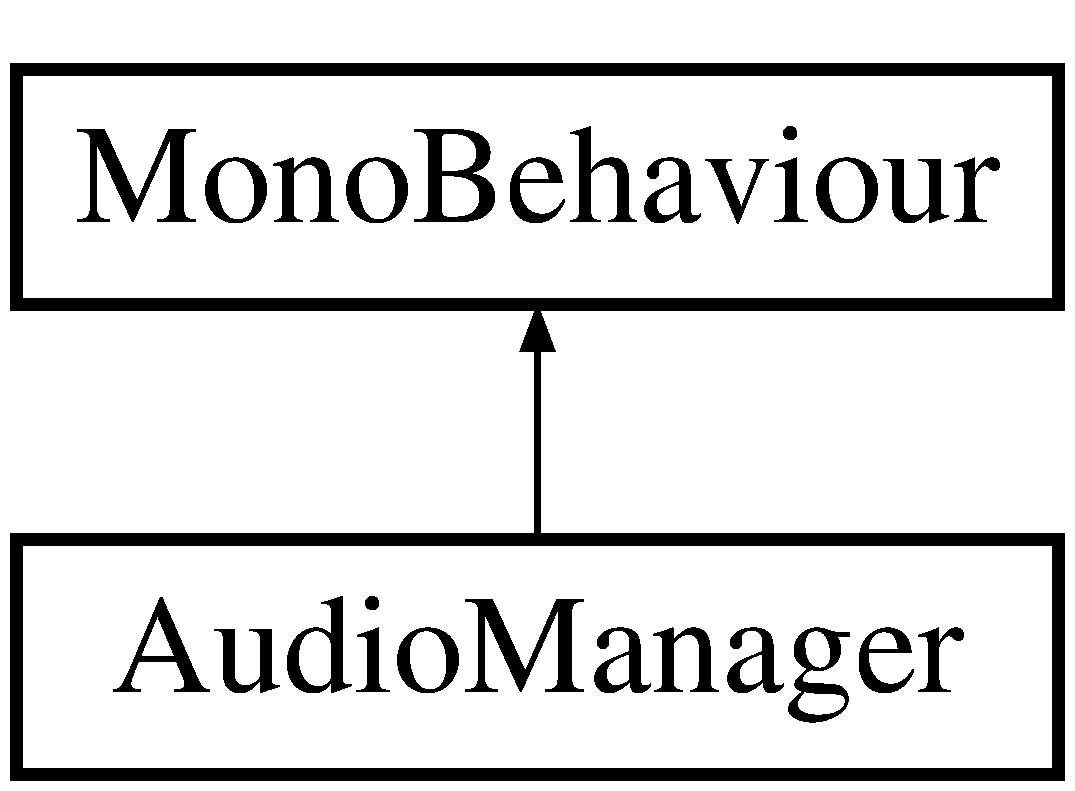
\includegraphics[height=2.000000cm]{class_audio_manager}
\end{center}
\end{figure}
\subsection*{Public Member Functions}
\begin{DoxyCompactItemize}
\item 
void \hyperlink{class_audio_manager_af2945459043f0a7f3f58f808903f587e}{Change\+B\+GM} (Audio\+Clip music)
\begin{DoxyCompactList}\small\item\em zmiana utworu \end{DoxyCompactList}\end{DoxyCompactItemize}
\subsection*{Public Attributes}
\begin{DoxyCompactItemize}
\item 
\mbox{\Hypertarget{class_audio_manager_a4a0d8e7375e1dcce42f53eb05bb8857b}\label{class_audio_manager_a4a0d8e7375e1dcce42f53eb05bb8857b}} 
Audio\+Source {\bfseries B\+GM}
\end{DoxyCompactItemize}


\subsection{Detailed Description}
Audio manager. 



\subsection{Member Function Documentation}
\mbox{\Hypertarget{class_audio_manager_af2945459043f0a7f3f58f808903f587e}\label{class_audio_manager_af2945459043f0a7f3f58f808903f587e}} 
\index{Audio\+Manager@{Audio\+Manager}!Change\+B\+GM@{Change\+B\+GM}}
\index{Change\+B\+GM@{Change\+B\+GM}!Audio\+Manager@{Audio\+Manager}}
\subsubsection{\texorpdfstring{Change\+B\+G\+M()}{ChangeBGM()}}
{\footnotesize\ttfamily void Audio\+Manager.\+Change\+B\+GM (\begin{DoxyParamCaption}\item[{Audio\+Clip}]{music }\end{DoxyParamCaption})}



zmiana utworu 


\begin{DoxyParams}{Parameters}
{\em music} & Music.\\
\hline
\end{DoxyParams}


The documentation for this class was generated from the following file\+:\begin{DoxyCompactItemize}
\item 
Assets/\+Scripts/\+Controllers/Audio\+Manager.\+cs\end{DoxyCompactItemize}

\hypertarget{class_audio_manager_check}{}\section{Audio\+Manager\+Check Class Reference}
\label{class_audio_manager_check}\index{Audio\+Manager\+Check@{Audio\+Manager\+Check}}


Audio manager sprawdzanie czy już jest muzyka.  


Inheritance diagram for Audio\+Manager\+Check\+:\begin{figure}[H]
\begin{center}
\leavevmode
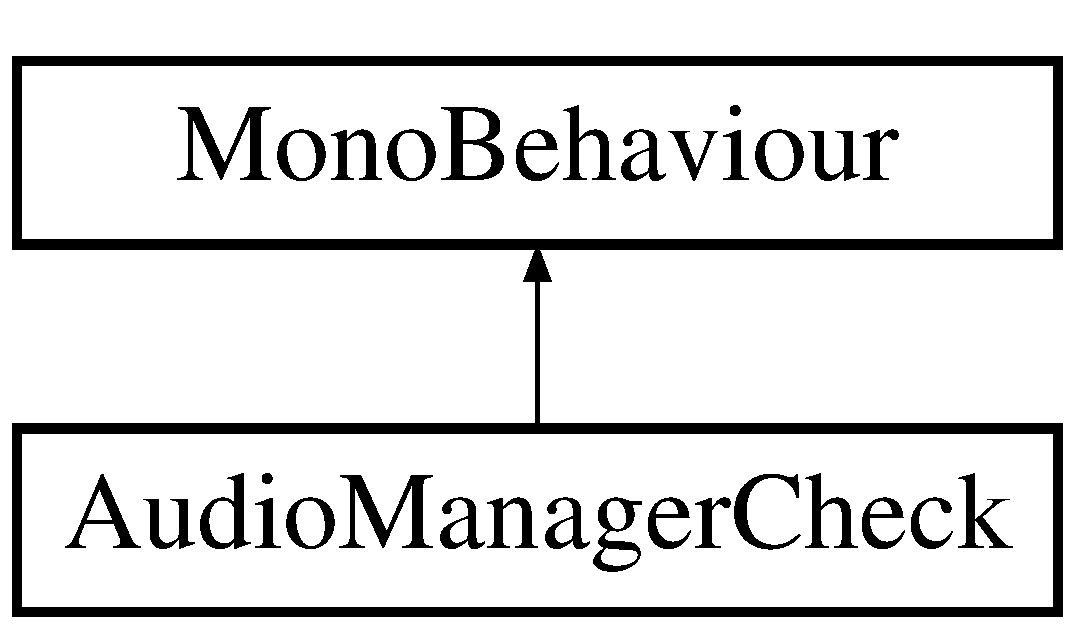
\includegraphics[height=2.000000cm]{class_audio_manager_check}
\end{center}
\end{figure}
\subsection*{Public Attributes}
\begin{DoxyCompactItemize}
\item 
\mbox{\Hypertarget{class_audio_manager_check_a7aa8709977e3b722d82f0ea416b6a305}\label{class_audio_manager_check_a7aa8709977e3b722d82f0ea416b6a305}} 
Game\+Object {\bfseries audio\+Man}
\end{DoxyCompactItemize}


\subsection{Detailed Description}
Audio manager sprawdzanie czy już jest muzyka. 



The documentation for this class was generated from the following file\+:\begin{DoxyCompactItemize}
\item 
Assets/\+Scripts/\+Controllers/Audio\+Manager\+Check.\+cs\end{DoxyCompactItemize}

\hypertarget{class_camera_follow}{}\section{Camera\+Follow Class Reference}
\label{class_camera_follow}\index{Camera\+Follow@{Camera\+Follow}}


Klasa dla kamery  


Inheritance diagram for Camera\+Follow\+:\begin{figure}[H]
\begin{center}
\leavevmode
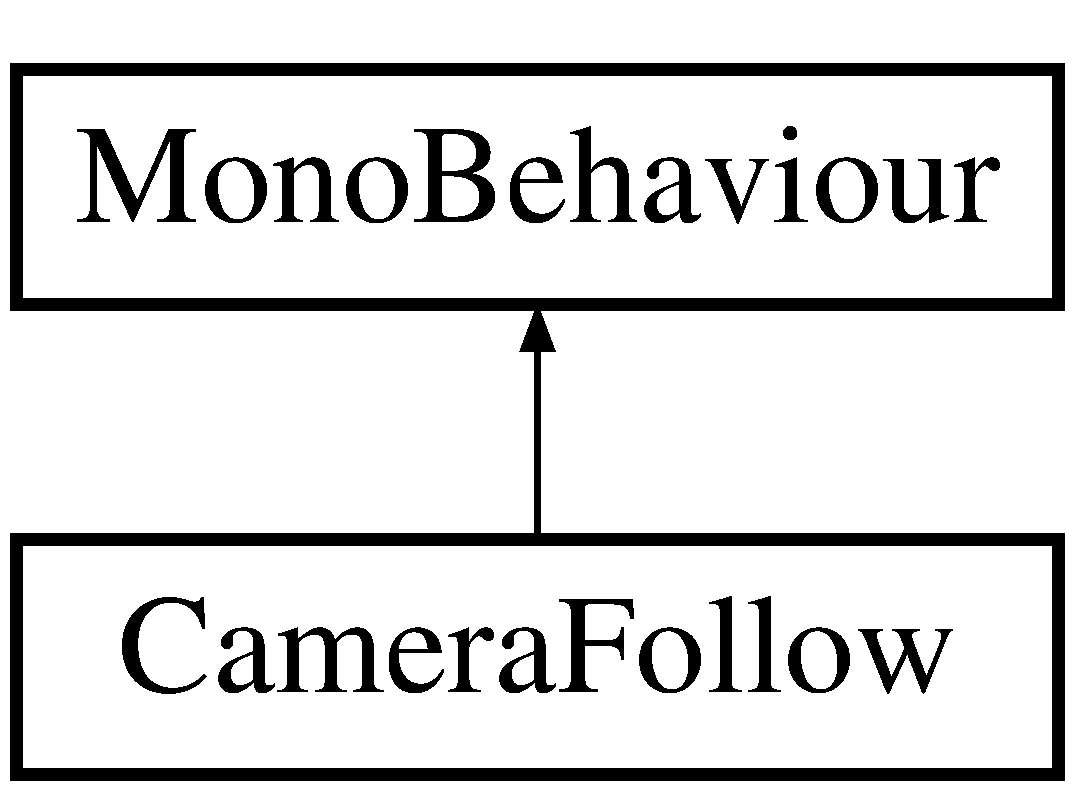
\includegraphics[height=2.000000cm]{class_camera_follow}
\end{center}
\end{figure}


\subsection{Detailed Description}
Klasa dla kamery 



The documentation for this class was generated from the following file\+:\begin{DoxyCompactItemize}
\item 
Assets/\+Scripts/\+Camera Scripts/Camera\+Follow.\+cs\end{DoxyCompactItemize}

\hypertarget{class_game_manager}{}\section{Game\+Manager Class Reference}
\label{class_game_manager}\index{Game\+Manager@{Game\+Manager}}


klasa ma 1 objekt całą gre i pomaga monitorować parametry  


Inheritance diagram for Game\+Manager\+:\begin{figure}[H]
\begin{center}
\leavevmode
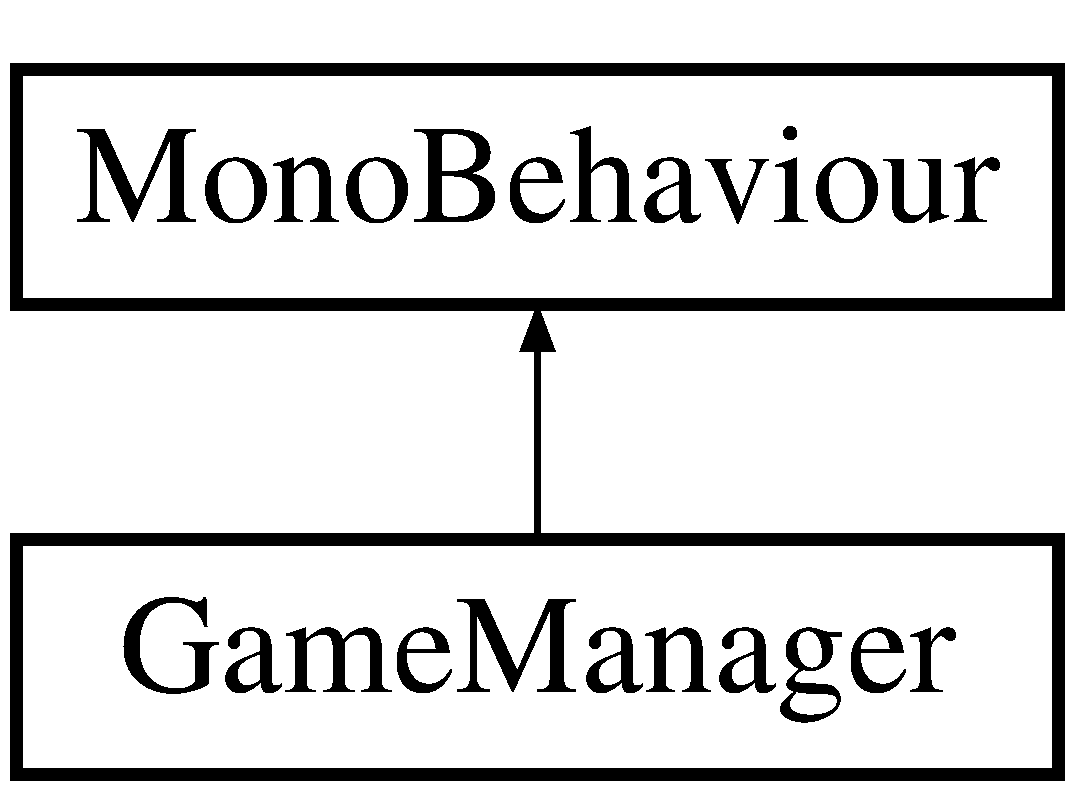
\includegraphics[height=2.000000cm]{class_game_manager}
\end{center}
\end{figure}
\subsection*{Public Attributes}
\begin{DoxyCompactItemize}
\item 
\mbox{\Hypertarget{class_game_manager_a8bbc0d69f19654f6072316716fa477e7}\label{class_game_manager_a8bbc0d69f19654f6072316716fa477e7}} 
double {\bfseries score}
\item 
\mbox{\Hypertarget{class_game_manager_ae9319015fb4e3a23a6d6fef6a7035964}\label{class_game_manager_ae9319015fb4e3a23a6d6fef6a7035964}} 
int {\bfseries lifescore}
\item 
\mbox{\Hypertarget{class_game_manager_a96156b85918560fe198febbcfec701b9}\label{class_game_manager_a96156b85918560fe198febbcfec701b9}} 
bool {\bfseries Hero\+Died\+And\+Restart}
\end{DoxyCompactItemize}
\subsection*{Static Public Attributes}
\begin{DoxyCompactItemize}
\item 
\mbox{\Hypertarget{class_game_manager_a7666e8468dac197b9eb32dd32128524f}\label{class_game_manager_a7666e8468dac197b9eb32dd32128524f}} 
static \hyperlink{class_game_manager}{Game\+Manager} {\bfseries instance}
\end{DoxyCompactItemize}


\subsection{Detailed Description}
klasa ma 1 objekt całą gre i pomaga monitorować parametry 



The documentation for this class was generated from the following file\+:\begin{DoxyCompactItemize}
\item 
Assets/\+Scripts/\+Controllers/Game\+Manager.\+cs\end{DoxyCompactItemize}

\hypertarget{class_gameplay_contoller}{}\section{Gameplay\+Contoller Class Reference}
\label{class_gameplay_contoller}\index{Gameplay\+Contoller@{Gameplay\+Contoller}}


Gameplay contoller.  


Inheritance diagram for Gameplay\+Contoller\+:\begin{figure}[H]
\begin{center}
\leavevmode
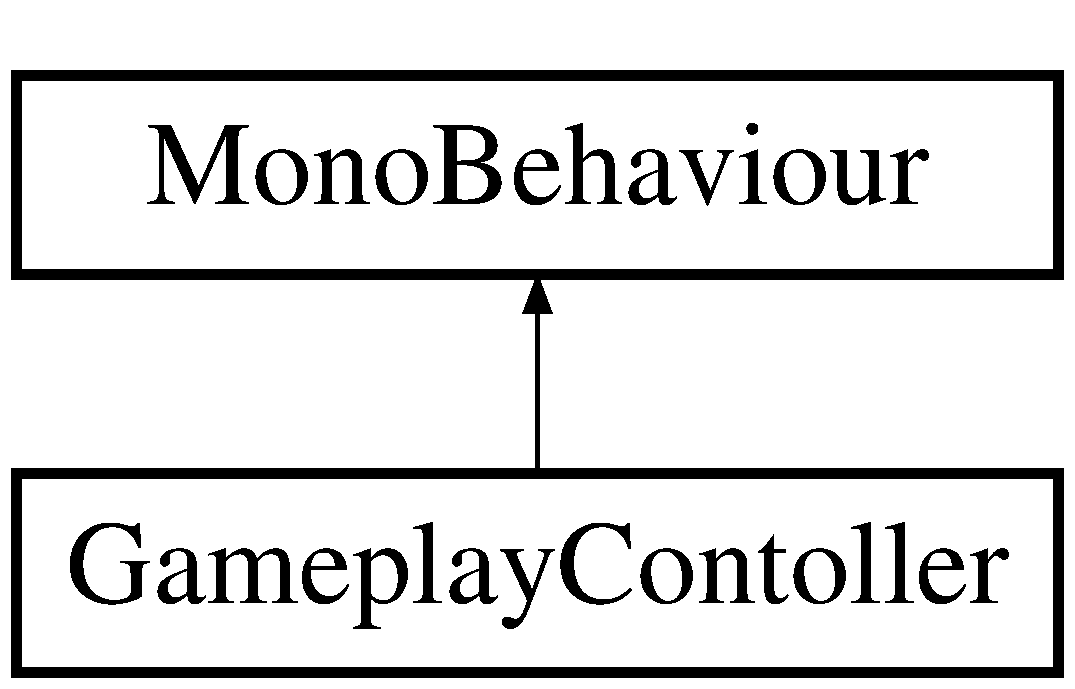
\includegraphics[height=2.000000cm]{class_gameplay_contoller}
\end{center}
\end{figure}
\subsection*{Public Member Functions}
\begin{DoxyCompactItemize}
\item 
void \hyperlink{class_gameplay_contoller_adfd4f2fbd55f084a0f1c5ddc2f5f3af6}{Increment\+Score} ()
\begin{DoxyCompactList}\small\item\em Increments the score. \end{DoxyCompactList}\item 
void \hyperlink{class_gameplay_contoller_a1de279d81704fd5035097275cb2d9519}{Decrement\+Life} ()
\begin{DoxyCompactList}\small\item\em Decrements the life. \end{DoxyCompactList}\end{DoxyCompactItemize}
\subsection*{Static Public Attributes}
\begin{DoxyCompactItemize}
\item 
\mbox{\Hypertarget{class_gameplay_contoller_ac5c3e93b39c20d0ea8cb59a994019fc7}\label{class_gameplay_contoller_ac5c3e93b39c20d0ea8cb59a994019fc7}} 
static \hyperlink{class_gameplay_contoller}{Gameplay\+Contoller} {\bfseries instance}
\end{DoxyCompactItemize}


\subsection{Detailed Description}
Gameplay contoller. 



\subsection{Member Function Documentation}
\mbox{\Hypertarget{class_gameplay_contoller_a1de279d81704fd5035097275cb2d9519}\label{class_gameplay_contoller_a1de279d81704fd5035097275cb2d9519}} 
\index{Gameplay\+Contoller@{Gameplay\+Contoller}!Decrement\+Life@{Decrement\+Life}}
\index{Decrement\+Life@{Decrement\+Life}!Gameplay\+Contoller@{Gameplay\+Contoller}}
\subsubsection{\texorpdfstring{Decrement\+Life()}{DecrementLife()}}
{\footnotesize\ttfamily void Gameplay\+Contoller.\+Decrement\+Life (\begin{DoxyParamCaption}{ }\end{DoxyParamCaption})}



Decrements the life. 

\mbox{\Hypertarget{class_gameplay_contoller_adfd4f2fbd55f084a0f1c5ddc2f5f3af6}\label{class_gameplay_contoller_adfd4f2fbd55f084a0f1c5ddc2f5f3af6}} 
\index{Gameplay\+Contoller@{Gameplay\+Contoller}!Increment\+Score@{Increment\+Score}}
\index{Increment\+Score@{Increment\+Score}!Gameplay\+Contoller@{Gameplay\+Contoller}}
\subsubsection{\texorpdfstring{Increment\+Score()}{IncrementScore()}}
{\footnotesize\ttfamily void Gameplay\+Contoller.\+Increment\+Score (\begin{DoxyParamCaption}{ }\end{DoxyParamCaption})}



Increments the score. 



The documentation for this class was generated from the following file\+:\begin{DoxyCompactItemize}
\item 
Assets/\+Scripts/\+Controllers/Gameplay\+Contoller.\+cs\end{DoxyCompactItemize}

\hypertarget{class_hero_walk}{}\section{Hero\+Walk Class Reference}
\label{class_hero_walk}\index{Hero\+Walk@{Hero\+Walk}}


Klasa dla utworzenia fizyki, biegu i etc. bohatera  


Inheritance diagram for Hero\+Walk\+:\begin{figure}[H]
\begin{center}
\leavevmode
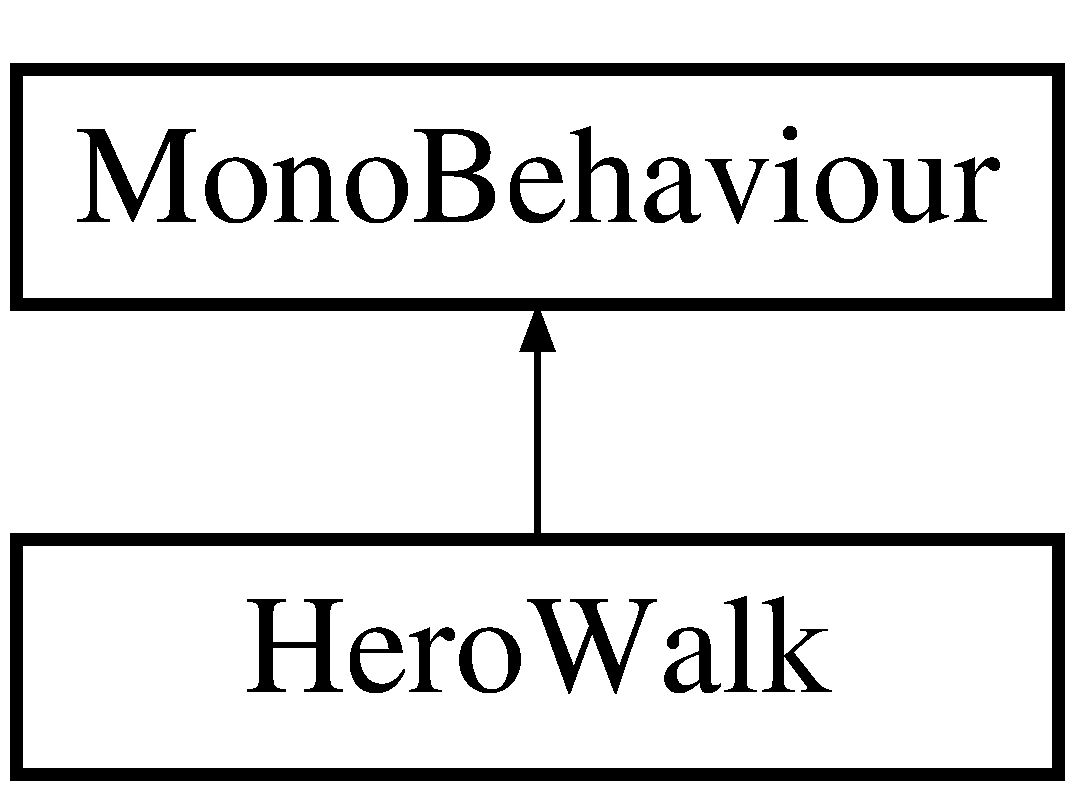
\includegraphics[height=2.000000cm]{class_hero_walk}
\end{center}
\end{figure}
\subsection*{Public Member Functions}
\begin{DoxyCompactItemize}
\item 
void \hyperlink{class_hero_walk_a438d7c97d2160c30063a1fddf50b7d71}{On\+Trigger\+Enter2D} (Collider2D collision)
\begin{DoxyCompactList}\small\item\em fizyka ziemi \end{DoxyCompactList}\end{DoxyCompactItemize}


\subsection{Detailed Description}
Klasa dla utworzenia fizyki, biegu i etc. bohatera 



\subsection{Member Function Documentation}
\mbox{\Hypertarget{class_hero_walk_a438d7c97d2160c30063a1fddf50b7d71}\label{class_hero_walk_a438d7c97d2160c30063a1fddf50b7d71}} 
\index{Hero\+Walk@{Hero\+Walk}!On\+Trigger\+Enter2D@{On\+Trigger\+Enter2D}}
\index{On\+Trigger\+Enter2D@{On\+Trigger\+Enter2D}!Hero\+Walk@{Hero\+Walk}}
\subsubsection{\texorpdfstring{On\+Trigger\+Enter2\+D()}{OnTriggerEnter2D()}}
{\footnotesize\ttfamily void Hero\+Walk.\+On\+Trigger\+Enter2D (\begin{DoxyParamCaption}\item[{Collider2D}]{collision }\end{DoxyParamCaption})}



fizyka ziemi 


\begin{DoxyParams}{Parameters}
{\em collision} & Collision.\\
\hline
\end{DoxyParams}


The documentation for this class was generated from the following file\+:\begin{DoxyCompactItemize}
\item 
Assets/\+Scripts/\+Hero Scripts/Hero\+Walk.\+cs\end{DoxyCompactItemize}

\hypertarget{class_main_menu_controller}{}\section{Main\+Menu\+Controller Class Reference}
\label{class_main_menu_controller}\index{Main\+Menu\+Controller@{Main\+Menu\+Controller}}


Klasa dla głownego menu  


Inheritance diagram for Main\+Menu\+Controller\+:\begin{figure}[H]
\begin{center}
\leavevmode
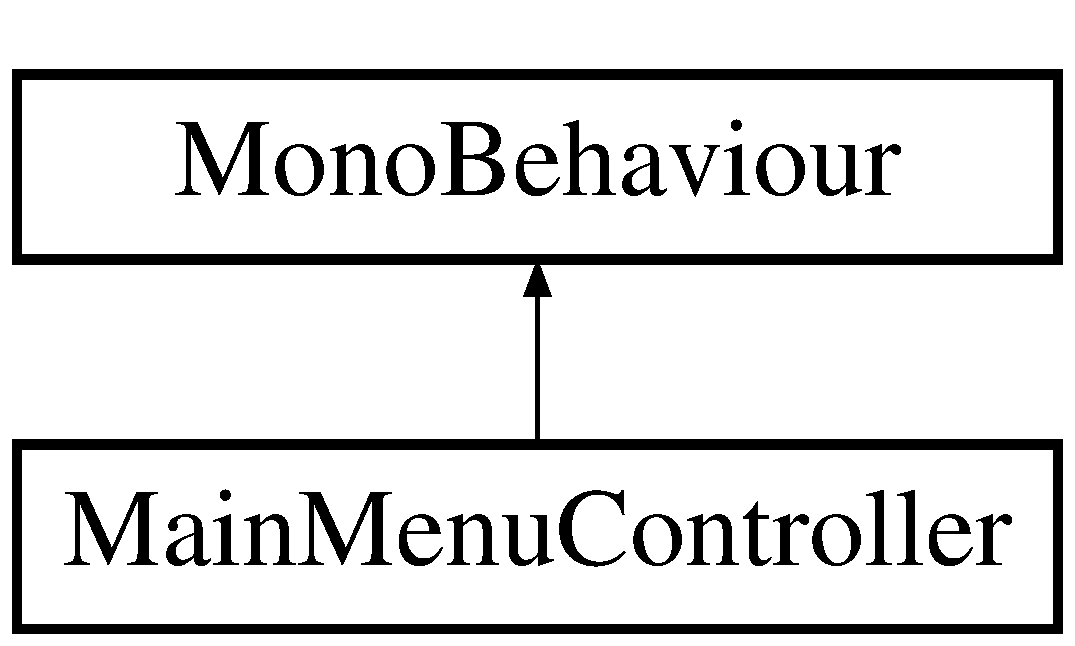
\includegraphics[height=2.000000cm]{class_main_menu_controller}
\end{center}
\end{figure}
\subsection*{Public Member Functions}
\begin{DoxyCompactItemize}
\item 
void \hyperlink{class_main_menu_controller_af693059f9f9b501929d35b23257f83ea}{Start\+Game} ()
\begin{DoxyCompactList}\small\item\em ładowanie 1 poziomu \end{DoxyCompactList}\item 
void \hyperlink{class_main_menu_controller_ab3774378b6ddd60fde78ecc9c2a5958e}{Load\+Level2} ()
\begin{DoxyCompactList}\small\item\em ładowanie 2 poziomu \end{DoxyCompactList}\item 
void \hyperlink{class_main_menu_controller_ab959d2affba0cdffd2d4c5cafba361ea}{Load\+Level3} ()
\begin{DoxyCompactList}\small\item\em ładowanie 3 poziomu \end{DoxyCompactList}\item 
void \hyperlink{class_main_menu_controller_ae7d63563e9950801e6b4e21250d723f6}{Back\+To\+Menu} ()
\begin{DoxyCompactList}\small\item\em ładowanie głownego menu \end{DoxyCompactList}\item 
void \hyperlink{class_main_menu_controller_ad03fe2e1403dbc61cbc2838abd0091f4}{Quit} ()
\begin{DoxyCompactList}\small\item\em wyjście \end{DoxyCompactList}\end{DoxyCompactItemize}


\subsection{Detailed Description}
Klasa dla głownego menu 



\subsection{Member Function Documentation}
\mbox{\Hypertarget{class_main_menu_controller_ae7d63563e9950801e6b4e21250d723f6}\label{class_main_menu_controller_ae7d63563e9950801e6b4e21250d723f6}} 
\index{Main\+Menu\+Controller@{Main\+Menu\+Controller}!Back\+To\+Menu@{Back\+To\+Menu}}
\index{Back\+To\+Menu@{Back\+To\+Menu}!Main\+Menu\+Controller@{Main\+Menu\+Controller}}
\subsubsection{\texorpdfstring{Back\+To\+Menu()}{BackToMenu()}}
{\footnotesize\ttfamily void Main\+Menu\+Controller.\+Back\+To\+Menu (\begin{DoxyParamCaption}{ }\end{DoxyParamCaption})}



ładowanie głownego menu 

\mbox{\Hypertarget{class_main_menu_controller_ab3774378b6ddd60fde78ecc9c2a5958e}\label{class_main_menu_controller_ab3774378b6ddd60fde78ecc9c2a5958e}} 
\index{Main\+Menu\+Controller@{Main\+Menu\+Controller}!Load\+Level2@{Load\+Level2}}
\index{Load\+Level2@{Load\+Level2}!Main\+Menu\+Controller@{Main\+Menu\+Controller}}
\subsubsection{\texorpdfstring{Load\+Level2()}{LoadLevel2()}}
{\footnotesize\ttfamily void Main\+Menu\+Controller.\+Load\+Level2 (\begin{DoxyParamCaption}{ }\end{DoxyParamCaption})}



ładowanie 2 poziomu 

\mbox{\Hypertarget{class_main_menu_controller_ab959d2affba0cdffd2d4c5cafba361ea}\label{class_main_menu_controller_ab959d2affba0cdffd2d4c5cafba361ea}} 
\index{Main\+Menu\+Controller@{Main\+Menu\+Controller}!Load\+Level3@{Load\+Level3}}
\index{Load\+Level3@{Load\+Level3}!Main\+Menu\+Controller@{Main\+Menu\+Controller}}
\subsubsection{\texorpdfstring{Load\+Level3()}{LoadLevel3()}}
{\footnotesize\ttfamily void Main\+Menu\+Controller.\+Load\+Level3 (\begin{DoxyParamCaption}{ }\end{DoxyParamCaption})}



ładowanie 3 poziomu 

\mbox{\Hypertarget{class_main_menu_controller_ad03fe2e1403dbc61cbc2838abd0091f4}\label{class_main_menu_controller_ad03fe2e1403dbc61cbc2838abd0091f4}} 
\index{Main\+Menu\+Controller@{Main\+Menu\+Controller}!Quit@{Quit}}
\index{Quit@{Quit}!Main\+Menu\+Controller@{Main\+Menu\+Controller}}
\subsubsection{\texorpdfstring{Quit()}{Quit()}}
{\footnotesize\ttfamily void Main\+Menu\+Controller.\+Quit (\begin{DoxyParamCaption}{ }\end{DoxyParamCaption})}



wyjście 

\mbox{\Hypertarget{class_main_menu_controller_af693059f9f9b501929d35b23257f83ea}\label{class_main_menu_controller_af693059f9f9b501929d35b23257f83ea}} 
\index{Main\+Menu\+Controller@{Main\+Menu\+Controller}!Start\+Game@{Start\+Game}}
\index{Start\+Game@{Start\+Game}!Main\+Menu\+Controller@{Main\+Menu\+Controller}}
\subsubsection{\texorpdfstring{Start\+Game()}{StartGame()}}
{\footnotesize\ttfamily void Main\+Menu\+Controller.\+Start\+Game (\begin{DoxyParamCaption}{ }\end{DoxyParamCaption})}



ładowanie 1 poziomu 



The documentation for this class was generated from the following file\+:\begin{DoxyCompactItemize}
\item 
Assets/\+Scripts/\+Controllers/Main\+Menu\+Controller.\+cs\end{DoxyCompactItemize}

\hypertarget{class_pause}{}\section{Pause Class Reference}
\label{class_pause}\index{Pause@{Pause}}


Klasa dla menu pause pod czas gry  


Inheritance diagram for Pause\+:\begin{figure}[H]
\begin{center}
\leavevmode
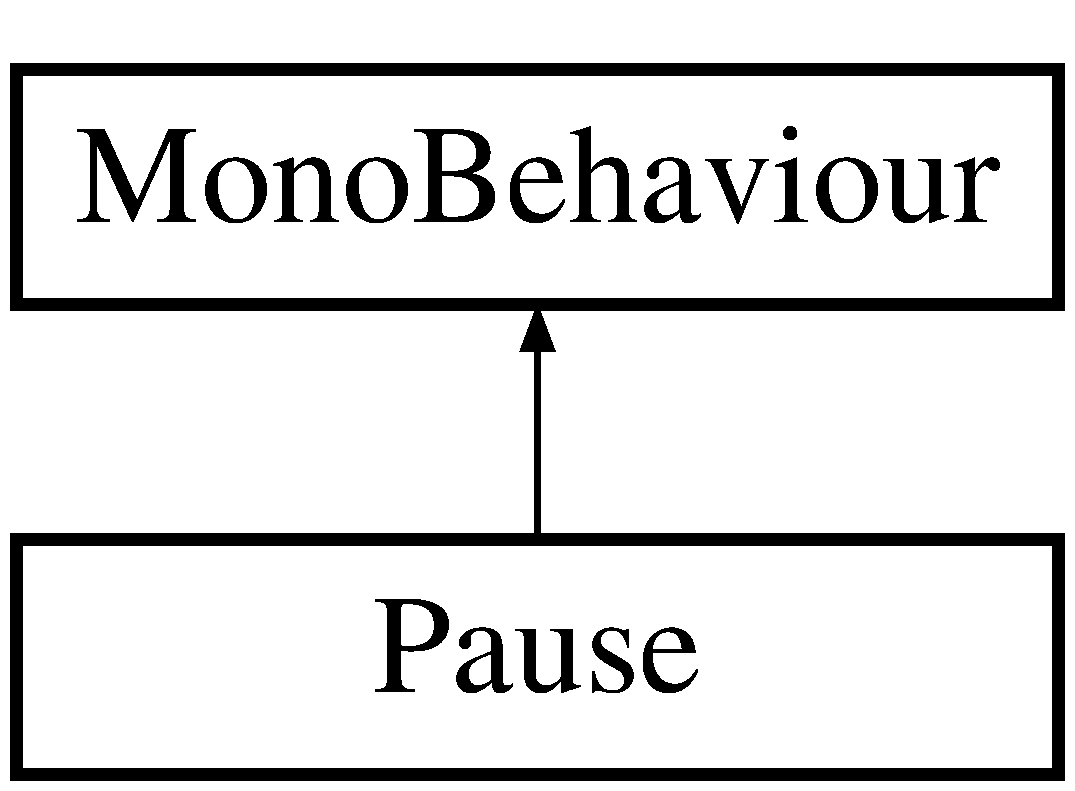
\includegraphics[height=2.000000cm]{class_pause}
\end{center}
\end{figure}
\subsection*{Public Member Functions}
\begin{DoxyCompactItemize}
\item 
void \hyperlink{class_pause_a1d1652c23fb2bab829e6d3f7e76727ec}{Resume} ()
\begin{DoxyCompactList}\small\item\em inicjalizacja resume \end{DoxyCompactList}\item 
void \hyperlink{class_pause_a5371367a048d854eba46cf8e2d746776}{Quit} ()
\begin{DoxyCompactList}\small\item\em inicjalizacja wyjścia \end{DoxyCompactList}\end{DoxyCompactItemize}
\subsection*{Public Attributes}
\begin{DoxyCompactItemize}
\item 
\mbox{\Hypertarget{class_pause_a7c21a7dd8cf53f8165e47d9af8821e54}\label{class_pause_a7c21a7dd8cf53f8165e47d9af8821e54}} 
Game\+Object {\bfseries Pause\+UI}
\end{DoxyCompactItemize}


\subsection{Detailed Description}
Klasa dla menu pause pod czas gry 



\subsection{Member Function Documentation}
\mbox{\Hypertarget{class_pause_a5371367a048d854eba46cf8e2d746776}\label{class_pause_a5371367a048d854eba46cf8e2d746776}} 
\index{Pause@{Pause}!Quit@{Quit}}
\index{Quit@{Quit}!Pause@{Pause}}
\subsubsection{\texorpdfstring{Quit()}{Quit()}}
{\footnotesize\ttfamily void Pause.\+Quit (\begin{DoxyParamCaption}{ }\end{DoxyParamCaption})}



inicjalizacja wyjścia 

\mbox{\Hypertarget{class_pause_a1d1652c23fb2bab829e6d3f7e76727ec}\label{class_pause_a1d1652c23fb2bab829e6d3f7e76727ec}} 
\index{Pause@{Pause}!Resume@{Resume}}
\index{Resume@{Resume}!Pause@{Pause}}
\subsubsection{\texorpdfstring{Resume()}{Resume()}}
{\footnotesize\ttfamily void Pause.\+Resume (\begin{DoxyParamCaption}{ }\end{DoxyParamCaption})}



inicjalizacja resume 



The documentation for this class was generated from the following file\+:\begin{DoxyCompactItemize}
\item 
Assets/\+Scripts/\+Controllers/Pause.\+cs\end{DoxyCompactItemize}

\hypertarget{class_player_score}{}\section{Player\+Score Class Reference}
\label{class_player_score}\index{Player\+Score@{Player\+Score}}


Player score.  


Inheritance diagram for Player\+Score\+:\begin{figure}[H]
\begin{center}
\leavevmode
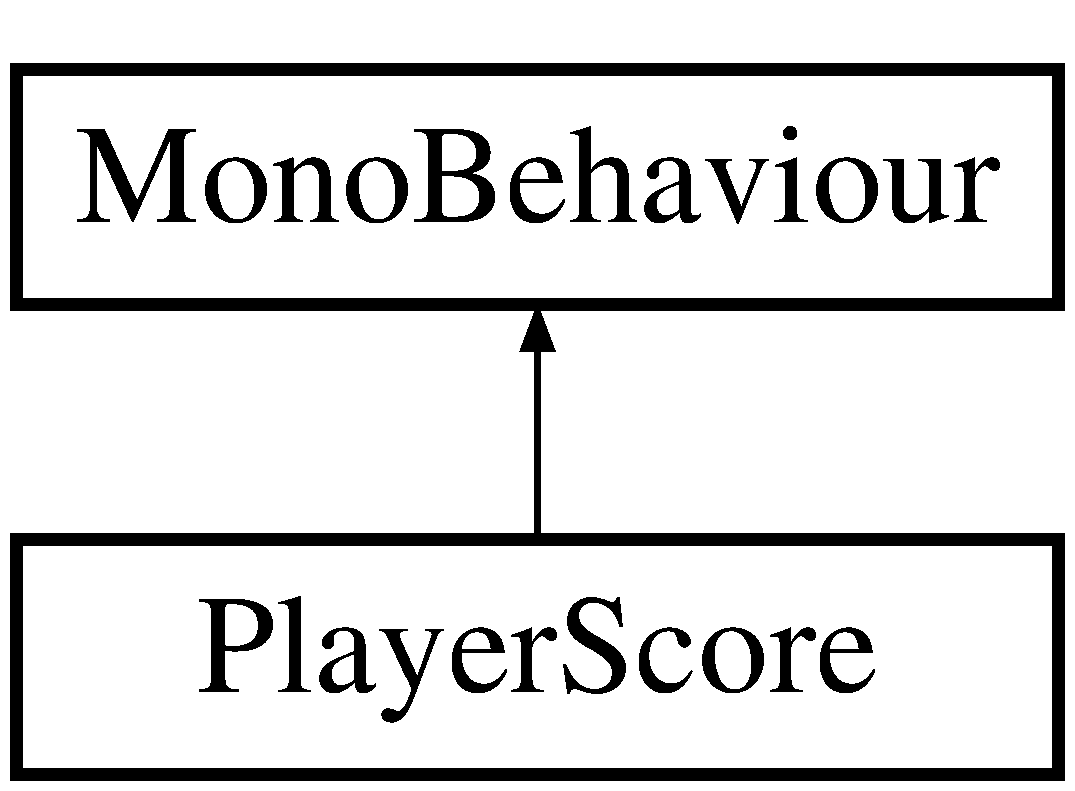
\includegraphics[height=2.000000cm]{class_player_score}
\end{center}
\end{figure}
\subsection*{Public Attributes}
\begin{DoxyCompactItemize}
\item 
\mbox{\Hypertarget{class_player_score_a571943554bd81ef392e8eb0a1504e94b}\label{class_player_score_a571943554bd81ef392e8eb0a1504e94b}} 
bool {\bfseries is\+Alive}
\end{DoxyCompactItemize}


\subsection{Detailed Description}
Player score. 



The documentation for this class was generated from the following file\+:\begin{DoxyCompactItemize}
\item 
Assets/\+Scripts/\+Hero Scripts/Player\+Score.\+cs\end{DoxyCompactItemize}

\hypertarget{class_skeleton_walk}{}\section{Skeleton\+Walk Class Reference}
\label{class_skeleton_walk}\index{Skeleton\+Walk@{Skeleton\+Walk}}


Klasa fizyki wrogów  


Inheritance diagram for Skeleton\+Walk\+:\begin{figure}[H]
\begin{center}
\leavevmode
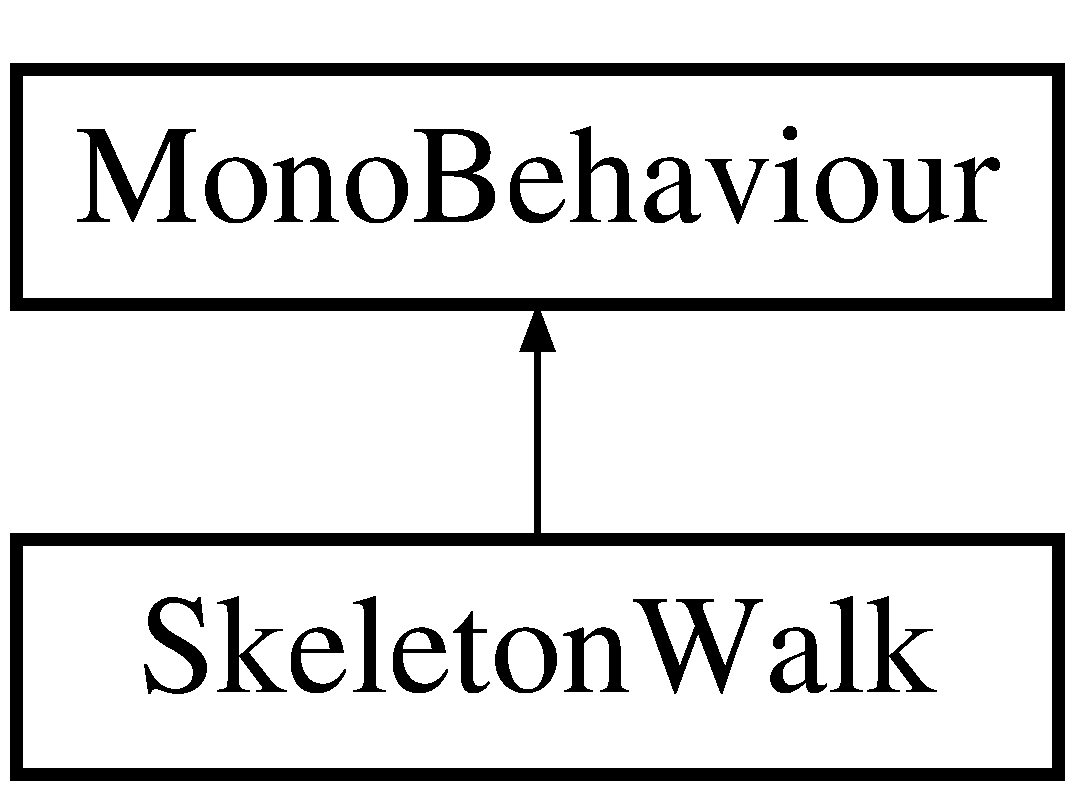
\includegraphics[height=2.000000cm]{class_skeleton_walk}
\end{center}
\end{figure}
\subsection*{Public Attributes}
\begin{DoxyCompactItemize}
\item 
\mbox{\Hypertarget{class_skeleton_walk_af73af7e0b7abbfc76713ea91b9ad9817}\label{class_skeleton_walk_af73af7e0b7abbfc76713ea91b9ad9817}} 
bool {\bfseries walk\+Left}
\end{DoxyCompactItemize}


\subsection{Detailed Description}
Klasa fizyki wrogów 



The documentation for this class was generated from the following file\+:\begin{DoxyCompactItemize}
\item 
Assets/\+Scripts/\+Skeletons Scripts/\+Skeleton1/Skeleton\+Walk.\+cs\end{DoxyCompactItemize}

\hypertarget{class_switch_music}{}\section{Switch\+Music Class Reference}
\label{class_switch_music}\index{Switch\+Music@{Switch\+Music}}


Zmiana utworu  


Inheritance diagram for Switch\+Music\+:\begin{figure}[H]
\begin{center}
\leavevmode
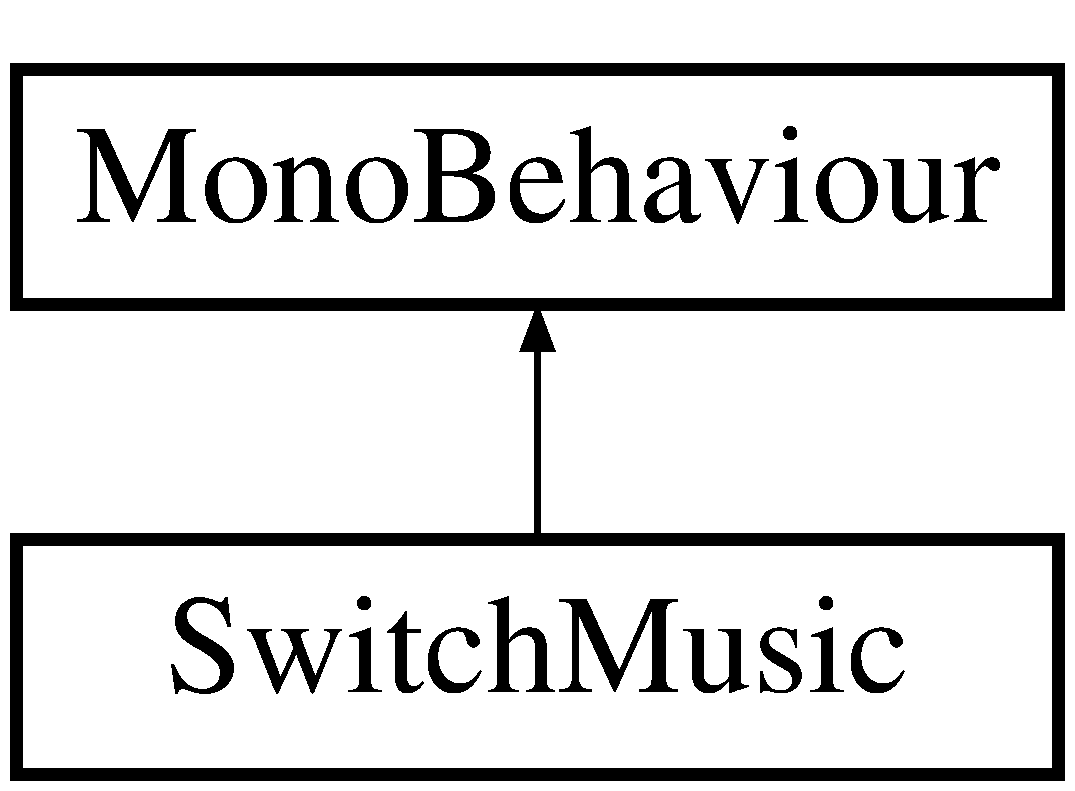
\includegraphics[height=2.000000cm]{class_switch_music}
\end{center}
\end{figure}
\subsection*{Public Attributes}
\begin{DoxyCompactItemize}
\item 
\mbox{\Hypertarget{class_switch_music_aaead7b595a4b2352367a4479f40f4981}\label{class_switch_music_aaead7b595a4b2352367a4479f40f4981}} 
Audio\+Clip {\bfseries New\+Track}
\end{DoxyCompactItemize}


\subsection{Detailed Description}
Zmiana utworu 



The documentation for this class was generated from the following file\+:\begin{DoxyCompactItemize}
\item 
Assets/\+Scripts/\+Controllers/Switch\+Music.\+cs\end{DoxyCompactItemize}

%--- End generated contents ---

% Index
\backmatter
\newpage
\phantomsection
\clearemptydoublepage
\addcontentsline{toc}{chapter}{Index}
\printindex

\end{document}
